\subsubsection{Fonctions à base radiale}
Nous désignerons un réseau de neurones \emph{fonctions à base radiale} par sa terminologie anglaise: \rbf pour \enum{Rasial Basis Function}.
\newcommand{\factnorm}{\sum_{r=1}^{m}x_{r}}
\ssstitle{Neurone}
Un neurone \textbf{caché} d'un \rbf n'effectue pas de somme pondérée de ses entrées.
Il applique directement sa fonction d'activation $\phi$, une gaussienne de moyenne $\mu$ et d'écart-type $\sigma$ où $x$, de dimension $n$, est l'entrée du neurone.
\begin{equation}\label{eq:cachephi}
 \phi(x) = e^{-\frac{1}{2}\sum_{k=1}^{n}\frac{(x_k-\mu_{ik})^2}{\sigma_{ik}^{2}}}
\end{equation}
Où $i$ est l'indice du neurone. $\mu$ s'appelle aussi \emph{prototype} dans le cas d'un \rbf.
%$\phi(x)$ peut se résumer en: \[\phi(x) = e^{-\beta||x-\mu||^2}\]Où $\beta$ est donc un coefficient qui règle la largeur de la courbe en cloche.\\
\\

Un neurone \textbf{de sortie} d'un \rbf n'effectue pas non plus de somme pondérée de ses entrées. Sa fonction d'activation est:
À une couche cachée, un \mlp peut déja servir pour la classification non linéaire.\cite{statistica}\\
\begin{equation}\label{eq:sortiephi}
 \phi(x) = \frac{\sum_{j=1}^{m}W_{ij}x_{j}}{\sum_{j=1}^{m}x_{j}}
\end{equation}
Où $i$ est l'indice du neurone et $x$ l'entrée de dimension $m$.
\begin{figure}
 \centering
 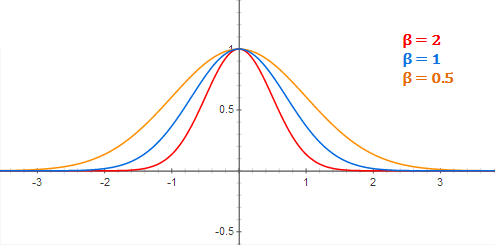
\includegraphics[scale=0.7]{../figures/RBFactivation.png}%TODO generer ça soit-même
 \caption{Activation d'un neurone RBF avec différentes valeurs d'écart-type}
 \label{rbfactivation}
\end{figure}
La Figure \ref{rbfactivation} représente la sortie d'un neurone \rbf où $\mu$ et $x$ sont de dimension 1 et $\mu = 0$.\\
Pour résumer, un neurone \rbf renvoie une valeur indiquant la simularité entre l'entrée et son prototype.
\ssstitle{Structure}
\begin{figure}
 \centering
 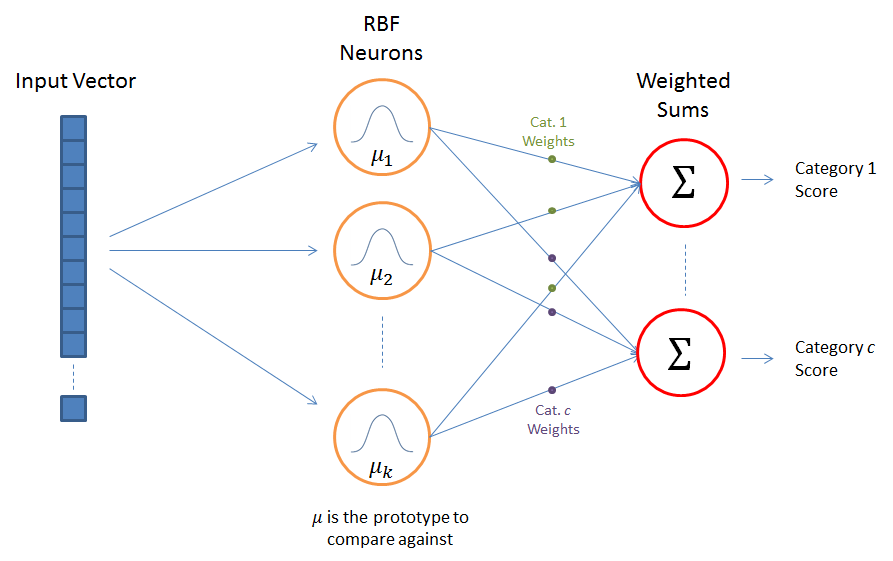
\includegraphics[scale=0.5]{../figures/RBFstruct.png}
 \caption{Structure RBF. \textbf{Source}: McCormick\cite{RBFtuto}}
 \label{structurerbf}
\end{figure}
La structure d'un \rbf est comme celle du \mlp sauf qu'il n'y a qu'une seule couche cachée (Figure \ref{structurerbf}).
\ssstitle{Apprentissage}
Dans ce réseau, les paramètres qui seront modifiés lors de l'apprentissage sont les poids des neurones de sortie et les moyennes et écart-types des neurones cachés.
L'algorithme de rétropropagation peut être utilisé pour un apprentissage supervisé d'un \rbf.
Reprenons \eqref{eq:Q}, l'erreur quadratique $Q$ défini dans la section \ref{sec:appmlp}.
En reprenant le même raisonnement que la rétropropagation dans un \mlp,
on va faire un pas de $\eta$ dans le sens opposé et proportionnel au gradient pour chaque poid $W_{ij}$ des neurones de sortie mais aussi des prototypes $\mu_i$ et écart-types $\sigma_i$ des neurones cachés.
C'est à dire que les paramètres seront modifiés de la sorte:
\begin{equation}%\label{eq:modifpoid}
 \Delta W_{ij} = -\eta \partiel{Q}{W_{ij}}
\end{equation}
\begin{equation}%\label{eq:modifmu}
 \Delta \mu_{ik} = -\eta \partiel{Q}{\mu_{ik}}
\end{equation}
\begin{equation}%\label{eq:modifsigma}
 \Delta \sigma_{ik} = \eta \partiel{Q}{\sigma_{ik}}
\end{equation}

Le dévellopement des formules de rétropropagation a été fait en annexe \ref{sec:eqrbf}.
Et voici ce que nous obtenons au final:\\
Pour un neurone de sortie :
\[\Delta W_{ij} = -\eta (\phi_i - s_i) \frac{x_j}{\factnorm}\]
Pour un neurone caché, posons $x_r$ l'entrée de $j$ provenant de $i$ (c'est à dire $\phi_i = x_r$),\\
posons $n$ la dimension de l'entrée de $j$,\\
posons aussi $R = \sum_{k=1}^{n}x_k$.
\[\Delta\mu_{ik} = -\eta \left[\sum_{i}(\phi_j - s_j) \frac{1}{R^2} \left(W_{jr}R - \sum_{k=1}^{n}W_{jk}x_k\right)\right] \phi_i\frac{x_k-\mu_{ik}}{\sigma_{ik}^2}\]
\[\Delta \sigma_{ik} = -\eta \left[\sum_{i}(\phi_j - s_j) \frac{1}{R^2} \left(W_{jr}R - \sum_{k=1}^{n}W_{jk}x_k\right)\right] \phi_i \frac{(x_k-\mu_{ik})^2}{\sigma_{ik}^3}\]

\ssstitle{Applications}
Un \rbf peut aussi servir pour la commande de robot.\cite{Gauthier}

Un des inconvénients des \rbf est que le nombre de neurones cachés croît avec la dimension et la taille du vecteur d'entrée puisqu'un neurone caché s'active seulement pour des entrées dans le voisinage de son prototype.
Nous pouvons raisonablement envisager ce modèle pour notre application puisque la description de l'état actuel et de l'état cible contiendra typiquement une coordonnée, un vecteur vitesse, une orientation et éventuellement l'accéleration, etc...
La taille de l'entrée sera donc relativement petite. Ce sera lors de la phase pratique qu'on évaluera le nombre de neurones cachés nécessaires.
De plus, les \rbf sont moins sensibles au bruit.\cite{adversarial}